\documentclass[a4paper]{report}
\usepackage[utf8]{inputenc}
\usepackage[polish]{babel}
\usepackage{polski}
\usepackage[margin=1in]{geometry}
\usepackage{caption}
\usepackage{color}
\usepackage{listings}
\usepackage{graphicx}

\linespread{1.3}

\begin{document}

\begin{center}

\textsc{\large Politechnika Warszawska}\\[0.1cm]
\textsc{\large Wydział Matematyki i Nauk Informacyjnych}\\[0.7cm]
\textsc{\Large Metody sztucznej inteligencji 2}\\[0.1cm]
\textsc{\large Raport z projektu}\\[0.5cm]
\textsc{\large Anna Zawadzka \& Piotr Waszkiewicz}\\[0.2cm]
{\large \today}\\[1cm]
\end{center}

\section{Opis projektu}

Projekt polega na realizacji zadania przedstawionego na stronie\\
\textit{https://www.physionet.org/challenge/2016}. Jego celem jest przetworzenie nagrań dźwięków serca i zidentyfikowanie, które z nich reprezentują zaburzoną pracę serca i wymagają diagnozy eksperta.\\
Fonokardiogram (\textit{Phonocardiogram},PCG) jest graficznym zapisem pracy serca. Poniższy rysunek przedstawia fragment zapisu PCG.\\\\

\begin{figure}[!htp]
    \centering
    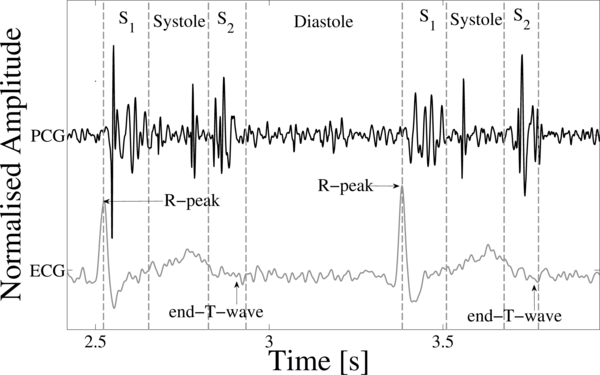
\includegraphics[scale=0.5]{figure1}
    \caption{Zapis PCG połączony z zapisem ECG}
    \label{figure1}
\end{figure}

Głównymi etapami zadania są:
\begin{itemize}
    \item Segmentacja nagrań na poszczególne części
    \item Wyodrębnienie cech sygnału
    \item Klasyfikacja obiektów na poprawne i zaburzone
\end{itemize}

Wraz z informacjami zamieszczonymi na stronie, dotyczącymi tematyki projektu, dołączone zostały zbiory nagrań audio pracy serca, oraz wstępny program realizujący cel zadania. Program ten zawiera wszystkie z wymienionych wcześniej etapów, jednak wymaga modyfikacji. \\
Użyta w implementacji segmentacja opisana jest przez autorów konkursu jako \textit{state of the art} i nie została przez nas zmieniona. Wyodrębniane cechy nie wyczerpują zakresu możliwych do wyekstrahowania informacji, dlatego też uzupełniliśmy istniejący zestaw o kilka nowych cech. W dostarczonym rozwiązaniu najgorzej jednak prezentuje się klasyfikacja, która wykorzystuje naiwne techniki statystyczne. To właśnie ona w pierwszym kroku została poddana usprawnieniom i poprawkom.\\

\section{Klasyfikatory}

\subsection{Opis}
Przy konstruowaniu lepszych klasyfikatorów rozważyliśmy kilka znanych i sprawdzonych metod: SVM, KNN i Lasy losowe. Wszystkie z wymienionych podejść charakteryzują się bardzo dobrymi wynikami w dziedzinie klasyfikacji, jednak niekoniecznie sprawdzają się równie dobrze w tych samych warunkach. W naszej pracy chcieliśmy zbadać wpływ wyboru klasyfikatora na skuteczność rozpoznawania zaburzeń rytmu serca w nagraniach. Testy zostały przeprowadzone z użyciem gotowej implementacji dostępnej na stronie konkursu.\\

\subsubsection{SVM}

Maszyna wektorów nośnych (SVM) jest klasyfikatorem którego nauka ma na celu wyznaczenie hiperpłaszczyzny rozdzielającej z maksymalnym marginesem przykłady należące do klas. Najprostszym sposobem jest próba liniowego odseparowania punktów. Niestety, często okazuje się, że jest ona niewystarczająca lub wręcz niemożliwa. W tym celu stworzone zostały funkcje jądrowe które mapują dostarczone punkty na odpowiadające im elementy z wyższych wymiarów celem umożliwienia ich późniejszej separacji. 

\begin{figure}[!htp]
	\centering
	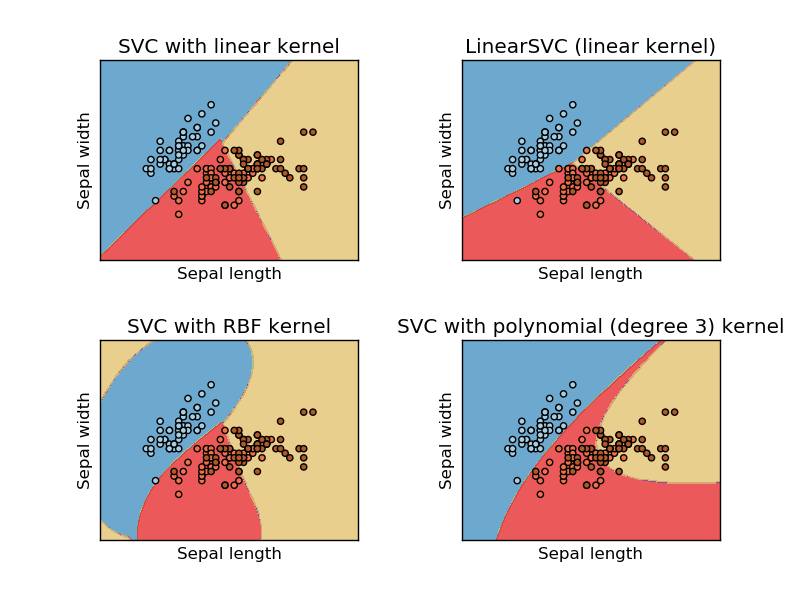
\includegraphics[scale=0.6]{svm.png}
	\caption{Przykład zachowania klasyfikatora SVM dla różnych funkcji jądrowych}
	\label{svmfigure}
\end{figure}


\subsubsection{RF}

\begin{figure}[!htp]
	\centering
	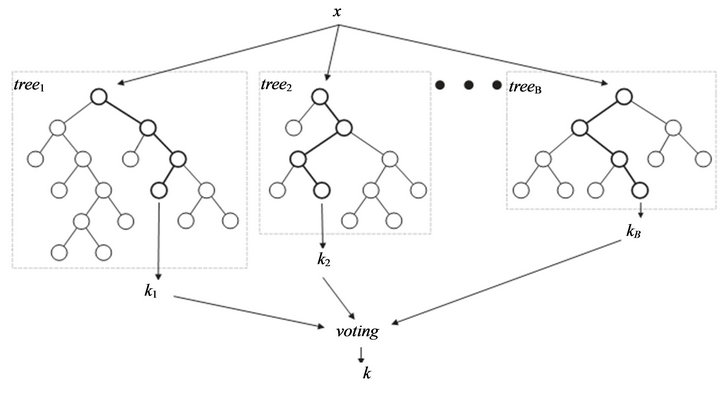
\includegraphics[scale=2.0]{rf.jpg}
	\caption{Klasyfikator korzystający z lasów losowych buduje odpowiednią liczbę drzew które następnie głosują nad zaklasyfikowaniem podanego elementu}
	\label{rffigure}
\end{figure}

\subsubsection{KNN}
Klasyfikacja metodą k-najbliższych sąsiadów polega na sprawdzeniu otoczenia wybranego punktu i nadanie mu przynależności do tej klasy do której należy większość sąsiadów. Liczba rozpatrywanych sąsiadów jest wartością arbitralną i jej zmiany mogą znacząco wpływać na jakość wyników.

\begin{figure}[!htp]
	\centering
	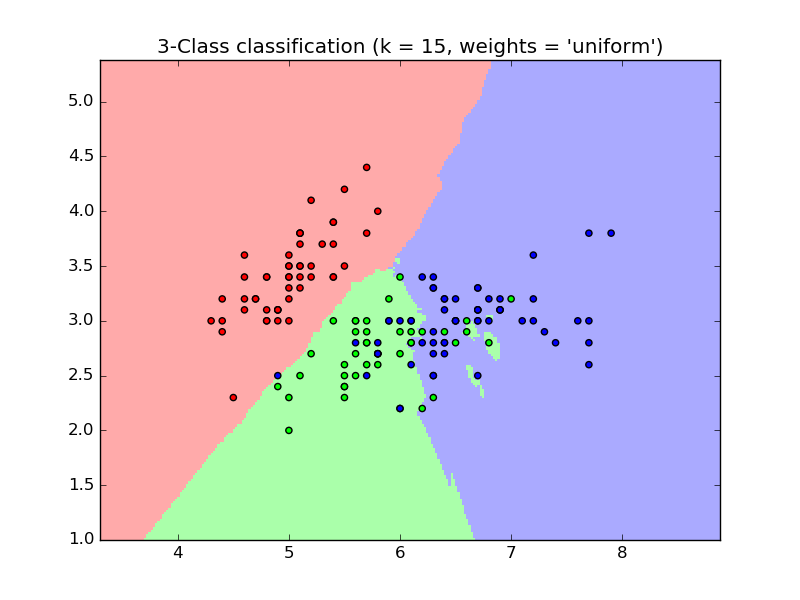
\includegraphics[scale=0.5]{knn.png}
	\caption{Klasyfikator KNN przydziela punktów do klas na podstawie ich odległości}
	\label{knnfigure}
\end{figure}

\subsection{Dobór parametrów}
Każdy z wybranych przez nas klasyfikatorów ma pewne charakterystyczne parametry, które odpowiednio dobrane skutkują najlepszą skutecznością. Aby zapewnić, że wybrane parametry rzeczywiście są najlepsze ich dobór nastąpił przy użyciu metody grid search. Jest to prosta koncepcyjnie metoda przeszukująca punkty na siatce w zdefiniowanej, ograniczonej przestrzeni potencjalnych wartości. Po jej zastosowaniu otrzymane zostały następujące wartości:
\begin{itemize}
	\item SVM: jądro: RBF (Gaussowskie)
	\item RF: liczba lasów = 100 
	\item KNN: liczba sąsiadów branych pod uwagę: 5
\end{itemize}

\section{Wyniki}
Wstępne testy przeprowadzone zostały na znormalizowanych cechach dostepnych w ramach dostarczonego przez konkurs oprogramowania. Zawierały one takie wartości jak odchylenia standardowe interwałów dla poszczególnych segmentów sygnału PCG, standardowe odchylenia oraz wartości średnie. Wyniki klasyfikacji zostały przedstawione w tabelce \ref{results1}. \\

\begin{table}[!htp]
    \centering
    \begin{tabular}{|r|l|}
      \hline 
      KNN & 0.29 \\
      \hline
      RF & 0.23 \\
      \hline
      SVM & 0.27 \\
      \hline
    \end{tabular} 
    
    \caption{Error ratio dla każdej z metod klasyfikacji dla znormalizowanych danych}
    \label{results1}
\end{table}

Próba uzyskania bardziej dokładnych klasyfikacji zakładała poszerzenie istniejącego wektora cech z 20 do 30 cech. Dodane zostały takie miary statyczne jak: różnica między wartością maksymalną a minimalną dla poszczególnych wartości z poprzedniego wektora cech oraz kurtozę tych pomiarów. Ponowne obliczenia doprowadziły do uzyskania takich wartości jakie zostały przedstawione w tabeli \ref{results2}.

\begin{table}[!htp]
    \centering
    \begin{tabular}{|r|l|}
      \hline 
      KNN & 0.32 \\
      \hline
      RF & 0.24 \\
      \hline
      SVM & 0.24 \\
      \hline
    \end{tabular} 
    
    \caption{Error ratio dla każdej z metod klasyfikacji dla danych z dodanymi nowymi cechami}
    \label{results2}
\end{table}

Oprócz standardowej klasyfikacji przy użyciu wspomnianych wcześniej narzędzi wykorzystane zostały narzędzia analizy statystycznej mającej na celu wykrycie anomalii. Ich celem było wykrycie najbardziej prawdopodobnych punktów leżących poza zbiorem "dobrych danych" które należy odrzucić. Te z punktów których przynależność do poszczególnych klas nie zgadzała się w przypadku klasyfikacji standardowymi narzędziami klasyfikującymi a wynikami z wykrycia anomalii uznawane były za zbyt zaszumione do poprawnej analizy (i liczące się w procesie zliczania błędów jako 0.5 błędu). Wyniki tego podejścia zaprezentowane zostały w tabelce \ref{results3}.

\begin{table}[!htp]
    \centering
    \begin{tabular}{|r|l|}
      \hline 
      KNN & 0.24 \\
      \hline
      RF & 0.25 \\
      \hline
      SVM & 0.25 \\
      \hline
    \end{tabular} 
    
    \caption{Error ratio dla każdej z metod klasyfikacji z uwzględnieniem anomalii}
    \label{results3}
\end{table}

Jak widać najbardziej na nowym podejściu skorzystała metoda KNNów. Wyniki dla SVMów i lasów losowych nieznaczenie się pogorszyły - jest to prawdopodobnie spowodowane sposobem liczenia punktów dla klasyfikacji. Nie są to jednak znaczne różnice i można powiedzieć, że metodę wykrywania anomalii warto wykorzystywać w połączeniu z KNNami.

\end{document}